\documentclass[../master.tex]{subfile}
\begin{document}

\section{Background}
In the previous course we have been working with another simplification of a game called Galaga. Here we were first introduced to the game-engine DIKUArcade, where the assignments from 4g and up to 7g, was partly used to make us learn how to make use of the game-engine. So we in this project would have easier creating and working on implementing the game \textit{Space Taxi}.\\

Space Taxi is an action game made for the Commodore 64, that is written by John Kutcher and published by Muse Software in 1984. This game simulates a flying taxi controlled by thrusters and which is being affected by the laws of physics. So when the ship flies upwards or to the left and right, the ship will accelerate gradually. When the player stops flying upwards the ship will start to fall by also accelerating gradually, and when the player starts thrusting upwards again it will de-accelerate gradually as well. The game is then about picking different costumers up and flying them to their desired destination pad, which can be on the same level or on another. The player will then earn some cash from the ride.\\

The onset of for the game of Space Taxi is basically a 40 x 23 grid, made from simple ASCII based text-file maps made into game levels:
\begin{figure}[h]
	\centering
	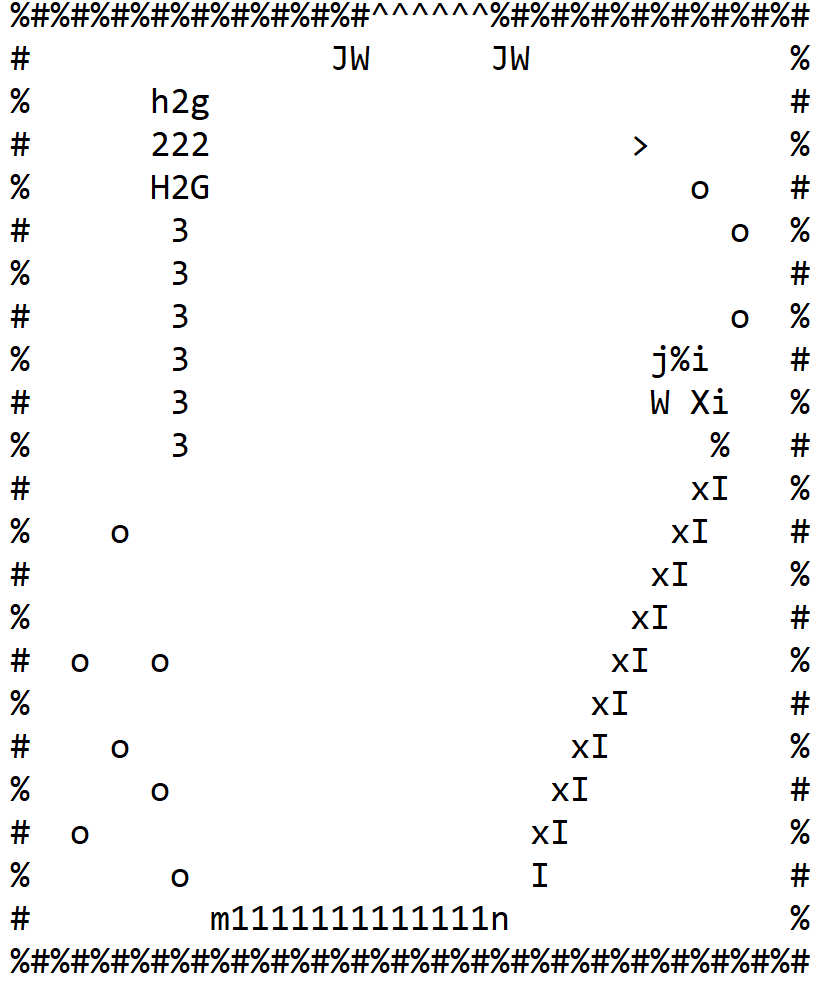
\includegraphics[width=0.35\textwidth]{./Pictures/ASCII.png}
    \caption{ASCII-File of Short-n-Sweet}
\end{figure}

\newpage

Then, one player will control the space taxi around the levels ``Short-n-Sweet`` and ``The-Beach'':
\begin{figure}[h]
	\centering
	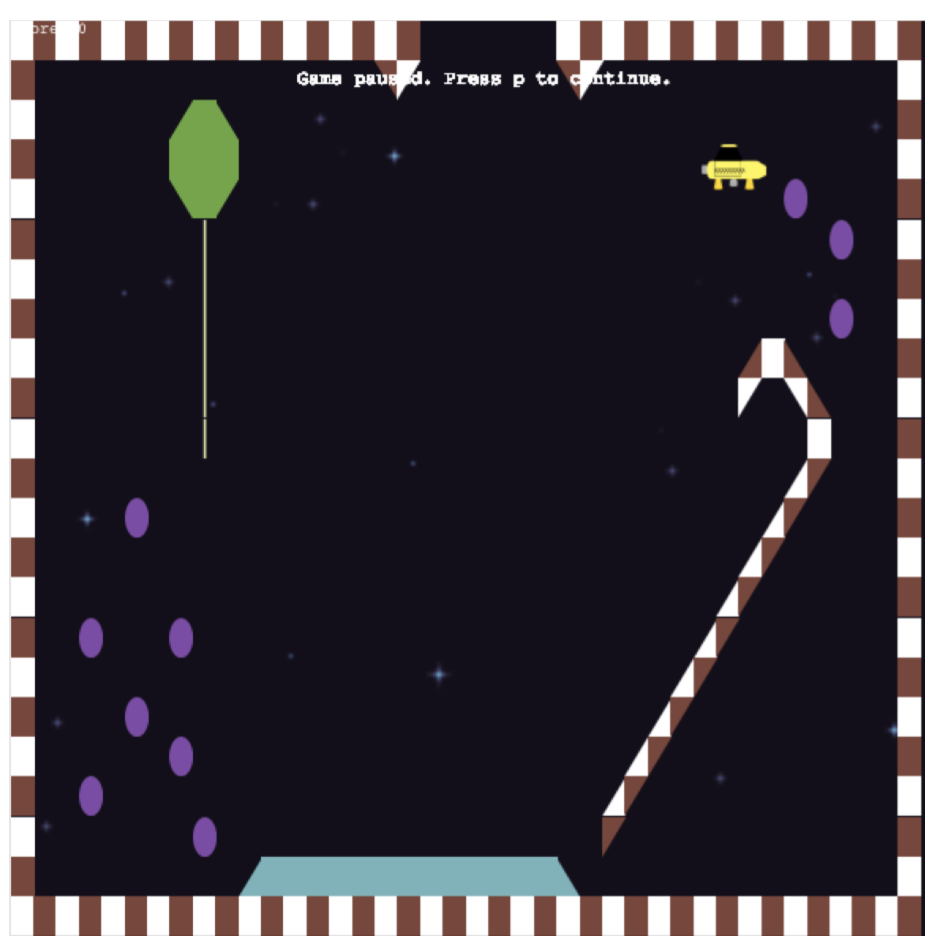
\includegraphics[width=0.45\textwidth]{./Pictures/GameLevel.png}
    \caption{Game level of Short-n-Sweet}
\end{figure}

The purpose of this project is not to showcase the DIKUArcade framework, but to learn how to produce a software product that meets some given specifications. The game may not be in the final state, but all the components should work as intended.\\

The development of our version of the game \textit{Space Taxi} was made over 4 parts, all comitted by a deliverable. In each of these deliverables where were different requirements there had to be met for passing the assignments. The process meeting these has been stated in our previous reports. In this final deliverable we will do the same, but this time we will be looking more at all the work we have done up until now. Our development process will focus more on delivering a code that will be easily readable and maintainable so it also can be further developed by other people, instead of adding new features. I.e. we will be focusing on refactoring and testing the code in this last deliverable.

<<<<<<< HEAD
\end{document}
=======

\end{document}



>>>>>>> 08b07d07f8721d17f006645a23da22c988ff10a9
